\section{Entity-Relationship Diagram}
An entity relationship diagram (ERD), also known as an entity relationship model, is a graphical representation of an information system that depicts the relationships among people, objects, places, concepts or events within that system. An ERD is a data modeling technique that can help define business processes and be used as the foundation for a relational database.\\
\subsection{Entity}
\begin{itemize}
\item Admin
\item User
\item Section
\item Products
\item Cart
\item Orders

\end{itemize}
\subsection{Attribute}
\begin{itemize}

\item Admin: AdminID, FirstName, LastName, Password
\item User: Email, FirstName, LastName, Password, UserID 
\item Section: SectionID, SectionName
\item Products: Quantity, Sizes, Description, Category, Price, SectionID, ProductCode, ProductName, ProductID, ImgLink, Bandname

\item Cart: Quantity, UserID, OrderID, ProductID, SubTotal, CartItemID
\item Orders: orderID, FirstName, PaymentMethod, Total, CartItemID, UserID, Adress, Phone, LastName 


\end{itemize}



 \subsection{Relationship}
 \begin{itemize}
  \item Admin manages Order
  \item Section contains product
  \item Cart contain product
  \item Order contains cart
  \item User places order

    \end{itemize}
   \subsection{Diagram}
   
   \begin{figure}
 \centering
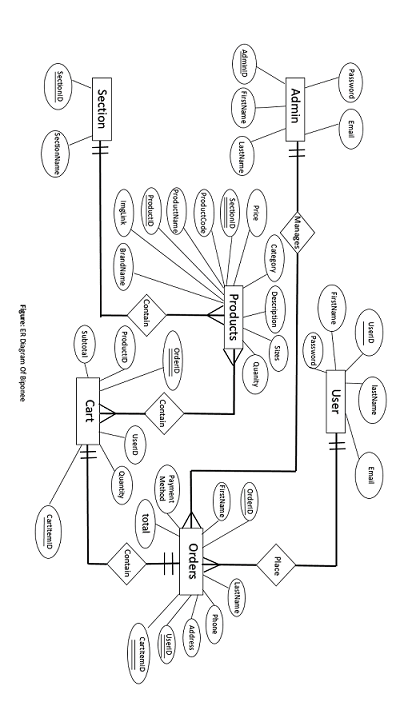
\includegraphics{figures/erdplus.png}
\caption{ERD of Biponee}
\end{figure}


\newpage

\section{Class Diagram}
Class diagrams are one of the most useful types of diagrams in UML as they clearly map out the structure of a particular system by modeling its classes, attributes, operations, and relationships between objects.\\


\subsection{Class}
\begin{itemize}
    \item User
    \item Admin
    \item ClothingsProduct
    \item Section
    \item Order
    \item Product
    \item CartItem
     \item OthersProduct
    
\end{itemize}


\subsection{Relationship}

\begin{itemize}
    \item Inheritance
    \item Association
    \item Aggregation
    \item Composition  
\end{itemize}
  
  
 \subsection{Multiplicity}
 \begin{itemize}
     \item 0 to 1 (Zero to one)
     \item 0...* (Zero to many) 
     \item 1...* (One to many)
     \item m...n (Specific number range)
     
 \end{itemize}
  \subsection{Diagram}
  \begin{figure}
 \centering
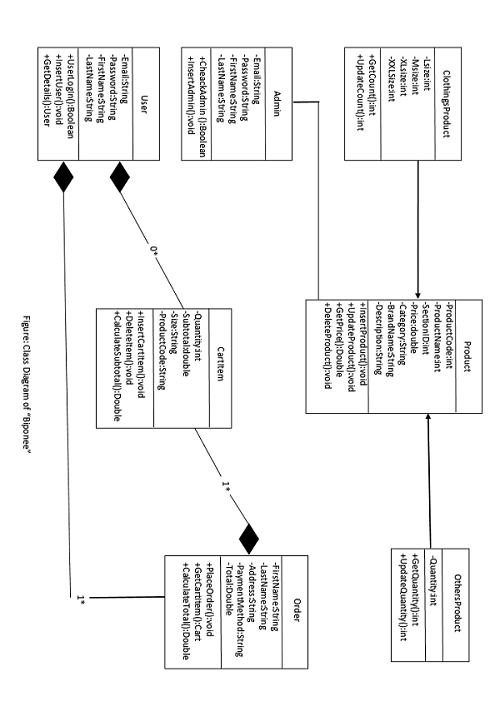
\includegraphics{figures/classfinal.png}
\caption{Class Diagram of Biponee}
\end{figure}


\newpage

\section{Conclusion}
 Entity relationship diagrams provide a visual starting point for database design that can also be used to help determine information system requirements throughout an organization. After a relational database is rolled out, an ERD can still serve as a referral point, should any debugging or business process re-engineering be needed later. We draw our ER Diagram which give us the clear Reflection of our project database.\\
 In Class Diagram a class defines the methods and variables in an object, which is a specific entity in a program or the unit of code representing that entity. Class diagrams are useful in all forms of object-oriented programming (OOP). 